\documentclass[UTF8]{ctexbeamer}

% 设置 Beamer 主题和配色
\usetheme{metropolis}
\usecolortheme[style=light]{Nord}
\usefonttheme[onlymath]{serif}
\metroset{
    numbering = fraction,
    sectionpage = progressbar,
    progressbar = frametitle
}

% 设置 \today 日期格式:YYYY-MM-DD
\usepackage{datetime2}

% 数学相关宏包
\usepackage{amsmath}
\usepackage{amssymb}
\usepackage{bm}
\usepackage{newtxmath}
\usepackage{cancel}

% 国际单位制
\usepackage{siunitx}


% 图表相关宏包
\usepackage{tabularx}
\usepackage{multirow}
\usepackage{booktabs}
\usepackage{subcaption}
\usepackage{graphicx}
\graphicspath{
    {../figure/}
    {../figures/}
}
\setbeamerfont{footnote}{size=\tiny}    % 脚注字号
\renewcommand{\thefootnote}{}           % 取消脚注编号
\renewcommand\arraystretch{1.25}        % 表格行高

\usepackage{tcolorbox}
\usepackage{hyperref}

% 预设一些好看的颜色
\definecolor{blue}{rgb}{0.1765,0.5216,0.9412}
\definecolor{red}{rgb}{0.9569,0.2627,0.2353}
\definecolor{yellow}{rgb}{1.0000,0.7373,0.1961}
\definecolor{green}{rgb}{0.0392,0.6588,0.3451}
\definecolor{pink}{rgb}{0.9843,0.4471,0.6000}
\definecolor{darkred}{rgb}{0.7490,0.2980,0.4157}
\definecolor{darkblue}{rgb}{0.3686, 0.5059, 0.6745}


% ===========================================================
\makeatletter
% 默认值
\renewcommand{\@title}{这里是报告的标题}
\renewcommand{\@date}{\today}
\renewcommand{\@author}{学生}
\newcommand{\@advisor}{导师}
\newcommand{\@school}{华中科技大学}
\renewcommand{\author}[1]{\renewcommand{\@author}{#1}}
\renewcommand{\date}[1]{\renewcommand{\@date}{#1}}
\renewcommand{\title}[1]{\renewcommand{\@title}{#1}}
\newcommand{\advisor}[1]{\renewcommand{\@advisor}{#1}}
\newcommand{\school}[1]{\renewcommand{\@school}{#1}}

\renewcommand{\maketitle}{
    \begin{frame}               % titlepage
        \thispagestyle{empty}
        \addtocounter{framenumber}{-1}
    
        \begin{center}
            \ {}
            \vspace{12mm}
    
            \begingroup         % title
            \zihao{3}\color{darkblue}\bfseries \@title
            \endgroup
    
            {\color{darkred}\rule{\textwidth}{0.7pt}}
    
            \vspace{3mm}
    
            \begin{tabular}{ll}
                报 \hfill 告 \hfill 人 & \@author \\
                指 \hfill 导 \hfill 老 \hfill 师 & \@advisor
            \end{tabular}
    
            \vspace{10mm}
    
            \@date \\
            {\small \@school}
        \end{center}
    \end{frame}
}
\makeatother

\newcommand{\theend}{
    \begin{frame}[standout]
        \zihao{0} 谢\ 谢\ !
    \end{frame}
}

\newcommand{\addtoc}{
    \begin{frame}{报告内容}
        \tableofcontents
    \end{frame}
}
% ===========================================================

\begin{document}
    
\begin{frame}               % titlepage
    \thispagestyle{empty}
    \addtocounter{framenumber}{-1}

    \begin{center}
        \ {}
        \vspace{12mm}

        \begingroup         % title
        \zihao{3}\color{darkblue}\bfseries 傅立叶变换与功率谱分析
        \endgroup

        {\color{darkred}\rule{\textwidth}{0.7pt}}

        \vspace{3mm}

        肖春雨

        \vspace{10mm}

        2021-12-02 \\
        {\small 华中科技大学}
    \end{center}
\end{frame}



\begin{frame}{报告内容}
    % \tableofcontents
    \begin{itemize}
        \setlength\itemsep{7pt}
        \item[$\color{darkblue}\bullet$] {\color{darkblue} 连续信号频域分析}
        \begin{itemize}
            \item 傅立叶级数:周期信号
            \item 傅立叶变换:非周期信号
            \item 两者的统一:狄拉克函数
        \end{itemize}

        \item[$\color{darkblue}\bullet$] {\color{darkblue} 离散信号频域分析}
        \begin{itemize}
            \item 时域采样:频率混叠
            \item 有限窗长:频率泄露
            \item 频域采样:栅栏效应
        \end{itemize}

        \item[$\color{darkblue}\bullet$] {\color{darkblue} 随机信号与功率谱估计}
        \begin{itemize}
            \item 功率谱密度:维纳-辛钦定理
            \item 谱估计算法:周期图、Welch、LPSD
            \item 功率谱应用:噪声评估、系统辨识
        \end{itemize}
    \end{itemize}
\end{frame}




\section{连续信号频域分析}

\begin{frame}{周期信号的频域分解}
    问题:如何将周期信号分解为正弦信号的叠加?

    \begin{figure}
        \centering
        \includegraphics[width=0.8\textwidth]{Fourier3d.pdf}
    \end{figure}

    \small
    \begin{tcolorbox}[boxrule=0.3pt,
        fontupper = \zihao{-5}\normalcolor]
        \begin{itemize}
            \item 选正交基:$\vec{x},\, \vec{y} \quad\rightarrow\quad \cos k \omega_0 t ,\, \sin k\omega_0 t$
            \item 坐标表示:$\vec{r} = r_x \vec{x} + r_y \vec{y}  \quad\rightarrow\quad f(t) = \sum a_n \cos  k \omega_0 t$
            \item 计算内积:$r_x = \sum r_i x_i \quad\rightarrow\quad a_k = \int f(t) \cos k \omega_0 t\, \mathrm{d}t$ 
        \end{itemize}
    \end{tcolorbox}
\end{frame}


\begin{frame}{单边傅立叶级数}
    综合公式
    \begin{equation*}
        x(t) = \frac{a_0}{2} + \sum_{k=1}^{+\infty} \left(a_k \cos k\omega_0t + b_k \sin k\omega_0t\right)
    \end{equation*}

    分析公式
    \begin{gather*}
        \left\{\begin{aligned}
            a_k &= \frac{2}{T} \int_T x(t) \cos k\omega_0t \,\mathrm{d}t \\
            b_k &= \frac{2}{T} \int_T x(t) \sin k\omega_0t \,\mathrm{d}t \\
        \end{aligned}\right.
    \end{gather*}

    收敛条件(Dirichlet Conditions)
    \begin{itemize}
        \item 周期内绝对可积
        \item 不存在第二类间断点
    \end{itemize}
\end{frame}



\begin{frame}{傅立叶级数及其性质}
    \begin{tcolorbox}[top=0mm,
        title = 傅立叶级数(Fourier Series),
        boxrule = 0.3pt,
        fontupper = \normalcolor\small]
        \begin{gather*}
            x(t) = \sum_{k=-\infty}^{+\infty} A_k \mathrm{e}^{\mathrm{j}k\omega_0t}  
            \qquad
            A_k = \frac{1}{T} \int_T x(t) \mathrm{e}^{-\mathrm{j}k\omega_0t}\,\mathrm{d}t
        \end{gather*}
    \end{tcolorbox}
    
    % \begin{columns}
    %     \begin{column}{0.4\textwidth}
    %         \centering
    %         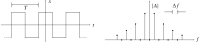
\includegraphics[width=\textwidth]{FourierSeries.pdf}
    %     \end{column}
    %     \begin{column}{0.5\textwidth}
    %         傅立叶级数的性质
    %         \begin{itemize}
    %             \item $\Delta f = {1}/{T}$
    %             \item 频谱共轭对称
    %             \item 周期 $\leftrightarrow$ 离散
    %         \end{itemize}
    %     \end{column}
    % \end{columns}
    \begin{figure}
        \centering
        \includegraphics[width=135pt]{FourierSeries1.pdf}
        \hspace{20pt}
        \includegraphics[width=135pt]{FourierSeries2.pdf}
    \end{figure}

    基本性质:
    频率间隔 $\Delta f = 1/T$,
    共轭对称, 
    周期 $\leftrightarrow$ 离散
\end{frame}


\begin{frame}{非周期信号}
    非周期信号 $\Leftrightarrow$ 周期无限大

    \begin{equation*}
        \begin{aligned}
            x(t) &= \sum_{k=-\infty}^{+\infty} A_k \mathrm{e}^{\mathrm{j}k\omega_0t}  \\
            &= \lim_{T \to \infty} \sum_{k=-\infty}^{+\infty} \frac{1}{T}\mathrm{e}^{\mathrm{j}k\omega_0t} 
            \underbrace{\int_{-\infty}^{+\infty} x(t) \mathrm{e}^{-\mathrm{j}k\omega_0t}\,\mathrm{d} t }_{X(\mathrm{j}\omega)} \\
            &= \lim_{\omega_0 \to 0} \sum_{k  = -\infty}^{+\infty} X(\mathrm{j}\omega) \mathrm{e}^{\mathrm{j}k\omega_0t} \omega_0  \\
            &= \int_{-\infty}^{+\infty} X(\mathrm{j}\omega)  \mathrm{e}^{\mathrm{j}\omega t}\, \mathrm{d}\omega
        \end{aligned}
    \end{equation*}
\end{frame}


\begin{frame}{傅立叶变换及其性质}
    \begin{tcolorbox}[top=0mm,
        title = 傅立叶变换(Fourier Transform),
        boxrule = 0.3pt,
        fontupper = \normalcolor\small]
        \begin{gather*}
            x(t) = \frac{1}{2\pi} \int_{-\infty}^{+\infty} X(\mathrm{j}\omega) \mathrm{e}^{\mathrm{j}\omega t}\,\mathrm{d}\omega 
            \qquad
            X(\mathrm{j}\omega) = \int_{-\infty}^{+\infty} x(t) \mathrm{e}^{-\mathrm{j}\omega t}\,\mathrm{d}t 
        \end{gather*}
    \end{tcolorbox}
    
    \begin{figure}
        \centering
        \includegraphics[width=135pt]{FourierTransform1.pdf}
        \hspace{20pt}
        \includegraphics[width=135pt]{FourierTransform2.pdf}
    \end{figure}

    基本性质:
    共轭对称, 
    非周期 $\leftrightarrow$ 连续
\end{frame}



\begin{frame}{狄拉克函数的引入}
    狄拉克函数(采样函数)
    \begin{equation*}
        u(t) = \left\{\begin{array}{cl}
            0 & t < 0 \\
            1 & t > 0
        \end{array}\right.
        \quad \rightarrow \quad
        \delta (t) := \frac{\mathrm{d}}{\mathrm{d}t} u(t) = \left\{\begin{array}{cl}
            \infty & t = 0 \\
            0 & t \ne 0
        \end{array}\right. 
    \end{equation*}

    \begin{itemize}
        \item 采样性质:$\int f(t) \delta (t-t_0) \, \mathrm{d} t = f(t_0)$
        \item 卷积性质:$\int f(\tau) \ast \delta (t-t_0-\tau) \, \mathrm{d} \tau = f(t-t_0)$
    \end{itemize}

    傅立叶变换的统一表达
    \begin{gather*}
        X(\mathrm{j}\omega) = 2 \pi A_k \delta (\omega - k\omega_0)\\
        \frac{1}{2\pi} \int_{-\infty}^{+\infty} X(\mathrm{j}\omega) \mathrm{e}^{\mathrm{j}\omega t}\,\mathrm{d}\omega 
        \Leftrightarrow  \sum_{k=-\infty}^{+\infty} A_k \mathrm{e}^{\mathrm{j}k\omega_0t}  
    \end{gather*}
\end{frame}



\section{离散信号频域分析}


\begin{frame}{时域采样与离散时间傅立叶变换}
    连续信号的离散化:冲击串采样 $p(t) = \sum \delta (t - n T_s) $

    \begin{figure}
        \centering
        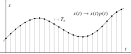
\includegraphics[width=200pt]{sample.pdf}
    \end{figure}
    \vspace{\fill}
    \begin{tcolorbox}[top=0mm,
        title = 离散时间傅立叶变换(Discrete-Time Fourier Transform),
        boxrule = 0.3pt,
        fontupper = \normalcolor\small]
        \begin{gather*}
            x(n) = \frac{1}{2\pi} \int_{2\pi} X(\mathrm{e}^{\mathrm{j}\omega}) \mathrm{e}^{\mathrm{j}\omega n}\,\mathrm{d}\omega 
            \qquad
            X(\mathrm{e}^{\mathrm{j}\omega}) = \sum_{n=-\infty}^{+\infty} x(n) \mathrm{e}^{-\mathrm{j}\omega n}            
        \end{gather*}
    \end{tcolorbox}
\end{frame}


\begin{frame}{连续信号采样与频谱混叠}
    \begin{columns}
        \begin{column}{0.55\textwidth}
            \centering
            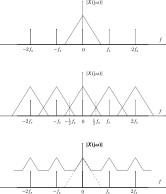
\includegraphics[width=\textwidth]{aliasing.pdf}
        \end{column}
        \begin{column}{0.4\textwidth}
            混叠的直接原因
            \begin{itemize}
                \item 高频噪声的影响
                \item 采样率太小
            \end{itemize}

            防止混叠的一般方法
            \begin{itemize}
                \item 抗混叠滤波器
                \item 提高采样率
            \end{itemize}
        \end{column}
    \end{columns}
\end{frame}


\begin{frame}{有限时间截断与频率泄漏}
    信号的加窗处理
    \begin{figure}
        \centering
        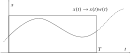
\includegraphics[height=70pt]{window.pdf}
        \hspace{20pt}
        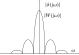
\includegraphics[height=70pt]{window-function.pdf}
    \end{figure}

    窗函数特性
    \begin{itemize}
        \item 主瓣宽度:频率分辨率 $f_\mathrm{res} = 1/T$ 
        \item 旁瓣高度:频率泄漏
    \end{itemize}

    常用窗函数:汉宁窗、海明窗、布莱克曼窗……
\end{frame}


\begin{frame}{离散傅立叶变换与栅栏效应}
    \begin{figure}
        \centering
        \includegraphics[width=260pt]{DFT.pdf}
    \end{figure}
    \vspace{\fill}
    \begin{tcolorbox}[top=0mm,
        title = 离散傅立叶变换(Discrete Fourier Transform) ,
        boxrule = 0.3pt,
        fontupper = \normalcolor\small]
        \begin{gather*}
            x(n) = \frac{1}{N} \sum_{k=0}^{N-1} X(k) \mathrm{e}^{\mathrm{j} 2\pi\frac{k}{N} n} 
            \qquad
            X(k) = \sum_{n=0}^{N-1} x(n) \mathrm{e}^{-\mathrm{j} 2\pi\frac{k}{N} n}            
        \end{gather*}
    \end{tcolorbox}
\end{frame}



\begin{frame}{频率分辨率与计算分辨率}
    频率分辨率: $X(\mathrm{j}\omega)$ 中能够分辨的最小频率间隔 $f_{\rm res} = \frac{1}{T}$
    
    计算分辨率:离散傅立叶变换的频率间隔(栅栏效应)$\Delta f = \frac{f_s}{N}$

    \begin{figure}
        \centering
        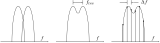
\includegraphics[width=0.9\textwidth]{freqs-resolution.pdf}
    \end{figure}

    \begin{itemize}
        \item 改善频率分辨率:增加采样时长
        \item 改善计算分辨率:增加采样时长、数据末尾补零
    \end{itemize}
    \footnote{程佩清. 数字信号处理. 第四版. 清华大学出版社. 2013. 185--189.}
\end{frame}


\section{随机信号与功率谱估计}


\begin{frame}{信号的频域特征}
    % 功率谱与幅度谱对比(单频信号 VS 带频信号)
\end{frame}



\begin{frame}{功率谱密度的计算}
    维纳--辛钦定理:功率谱密度是自相关函数的傅立叶变换
    \begin{align*}
        S_x(\omega) &= \int_{-\infty}^{+\infty} \left( \lim_{T \to \infty} \, \frac{1}{2T} \, \int_{-T}^{T} x(t-\tau)x(t) \,\mathrm{d} t   \right) \mathrm{e}^{-\mathrm{j}\omega\tau} \,\mathrm{d} \tau  \\
        &= \lim_{T \to \infty} \, \frac{1}{2T} \, \int_{-T}^{T} \int_{-\infty}^{+\infty} x(t)\mathrm{e}^{-\mathrm{j} \omega t} x(t-\tau)\mathrm{e}^{-\mathrm{j}\omega(\tau-t)} \,\mathrm{d} \tau \,\mathrm{d} t \\
        &= \lim_{T \to \infty} \, \frac{1}{2T} \, \int_{-T}^{T}  x(t)\mathrm{e}^{-\mathrm{j} \omega t} \bar{X}(\mathrm{j}\omega) \,\mathrm{d} t \\
        &= \lim_{T \to \infty} \, \frac{1}{2T} \, \left| X(\mathrm{j}\omega) \right|^2
    \end{align*}
    离散情况:$2T \rightarrow NT_s = N/f_s,\, X(\mathrm{j}\omega)\rightarrow X(k)/f_s$
\end{frame}


% 功率谱定义(方差 VS 幅值)

% 功率谱算法

\begin{frame}[standout]
    \zihao{0} 谢\ 谢\ !
\end{frame}


\end{document}